\subsection{Red-Black Tree - RBT}

\subsubsection{Concept}

A \textbf{Red-Black Tree} is a variation of the binary search tree that uses a set of properties to stay balanced. This guarantees that insertion, search, and deletion operations have logarithmic time complexity, even in the worst cases.

To ensure this balance, each node in the tree is assigned a color---either \textcolor{red}{red} or \textbf{black}---and after each modification (insertion or deletion), the tree's balance is restored through rotations and recolorings as needed.

A Red-Black Tree must obey the following properties:
\begin{enumerate}
    \item \underline{Node Color:} Every node is either red or black.
    \item \underline{Root Property:} The root of the tree is always black.
    \item \underline{Red Property:} A red node cannot have red children (i.e., there are no two consecutive red nodes on any path).
    \item \underline{Black Property:} Every path from a given node to any of its descendant NIL nodes contains the same number of black nodes.
    \item \underline{Leaf Property:} All leaves (NIL nodes) are black.
\end{enumerate}

\subsubsection{Implementation}

\begin{itemize}
    \item \underline{\textbf{Transplant Function:}}

    The \texttt{transplant} auxiliary function is responsible for replacing one node, $u$, with another node, $v$, in the tree. In other words, it makes the parent of $u$ point to $v$. Furthermore, if $v$ is not null, the function updates the parent pointer of $v$ to point to the former parent of $u$.

    \item \underline{\textbf{FixInsert Function:}}
    
    Given the properties of a Red-Black Tree, we first need to determine the color of the newly added node, which we will call $z$. As established, $z$ can only be black or red. Let's see what happens in each case:
    
    If $z$ is black: 
    \begin{itemize}
        \item It violates Property 4, unless $z$ is the root.
    \end{itemize}
    
    If $z$ is red:
    \begin{itemize}
        \item Property 4 is maintained.
        \item If its parent is red, Property 3 is violated.
        \item If it is the root, Property 2 is violated.
    \end{itemize}
    
    Therefore, by convention, every node initially inserted into a Red-Black Tree is colored red. When this insertion leads to a violation of the tree's properties, the issue can be resolved by handling a series of specific cases.
    
    In addressing these violations, three main cases (and their symmetric counterparts) are distinguished.
    \begin{itemize}
    \item \textit{\textbf{First Case:} The uncle of the newly inserted node $z$ is red.}

    Since $z$ is inserted as a red node, its parent, $p$, might also be red. This configuration violates the Red Property of a Red-Black Tree (a red node cannot have a red child). Assuming that the uncle of $z$, denoted by $y$, is also red, we perform a recoloring to fix the violation.

    In this situation, we assume that the grandparent of $z$, denoted by $g$, was black before the insertion---which guarantees the tree was valid up to that point. The fix consists of recoloring both $p$ and $y$ to black, and $g$ to red. This resolves the local conflict.

    However, this recoloring might have introduced a new conflict at the level of the grandparent, $g$, if its parent is also red. Therefore, the verification and correction must be applied recursively up the tree until all properties are restored.

        \begin{center}
        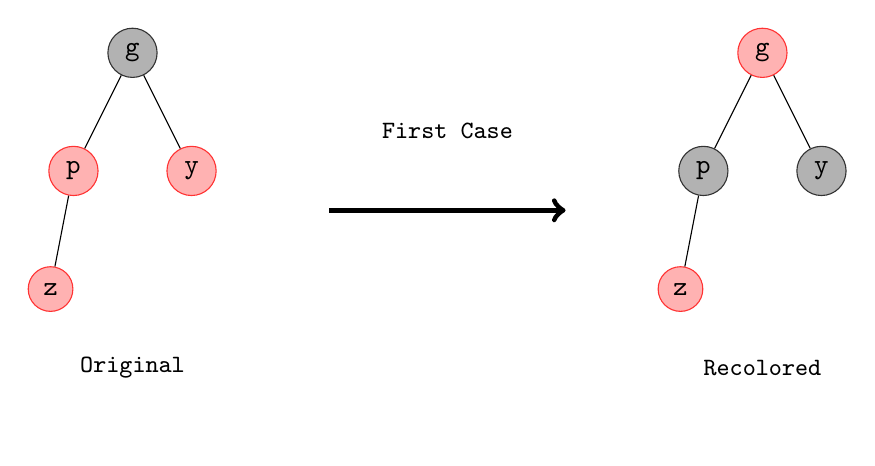
\begin{tikzpicture}[
          level distance=15mm, sibling distance=15mm,
          every node/.style={circle, draw, minimum size=8mm, font=\ttfamily\small}
        ]
        
        \begin{scope}[xshift=-4cm, every node/.style={circle, draw=blue!80, fill=blue!20, font =\ttfamily}]
            \node[circle, draw=black!80, fill=black!30] {g}
                child {node [circle, draw=red!80, fill=red!30]{p}
                    child[left] {
                        node [circle, draw=red!80, fill=red!30]{z}
                    } 
                }
                child{node[circle, draw=red!80, fill=red!30]{y}}
            ;
        \end{scope}
        
        \begin{scope}[xshift=4cm, every node/.style={circle, draw=blue!80, fill=blue!20, font=\ttfamily}]
            \node[circle, draw=red!80, fill=red!30] {g}
                child {node [circle, draw=black!80, fill=black!30]{p}
                    child[left] {
                        node [circle, draw=red!80, fill=red!30]{z}
                    } 
                }
                child{node[circle, draw=black!80, fill=black!30]{y}}
            ;
        \end{scope}
        
        \draw[->, very thick, line width=2pt] (-1.5,-2.0) -- (1.5,-2.0) 
            node[midway, above, yshift=0.2pt, draw=none, fill=none] {First Case};
        
                \node[draw=none, fill=none] at (-4, -4) {\textbf{Original} };
        \node[draw=none, fill=none] at (4, -4) {\textbf{Recolored} };
        
        \end{tikzpicture}
        \end{center} 
        \item \textit{\textbf{Second Case:} The uncle is black and the inserted node is a right child.}

        In this scenario, node $z$ is inserted as red, its parent $p$ is also red, while the uncle is black. Furthermore, $z$ is a right child of $p$, and $p$ is a left child of the grandparent, $g$.

        Since the uncle is black, we cannot resolve the issue with a simple recoloring. To handle the imbalance created by $z$'s position as a right child, we apply a \textbf{left rotation} on its parent, $p$. This rotation transforms the current problem into the configuration of the \textbf{Third Case}, which is simpler to resolve.

        This rotation repositions the nodes, effectively preparing the structure for the final adjustments described in the next step.
        \begin{center}
        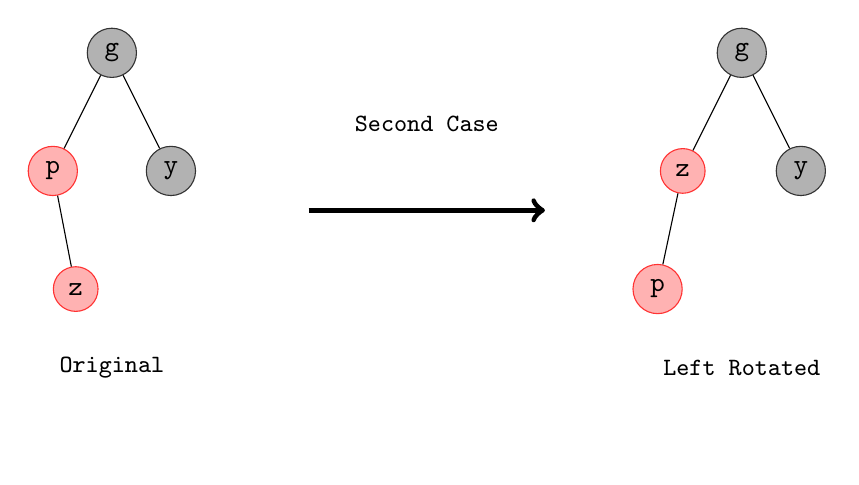
\begin{tikzpicture}[
          level distance=15mm, sibling distance=15mm,
          every node/.style={circle, draw, minimum size=8mm, font=\ttfamily\small}
        ]
        
        \begin{scope}[xshift=-4cm, every node/.style={circle, draw=blue!80, fill=blue!20, font =\ttfamily}]
            \node[circle, draw=black!80, fill=black!30] {g}
                child {node [circle, draw=red!80, fill=red!30]{p}
                    child[right] {
                        node [circle, draw=red!80, fill=red!30]{z}
                    } 
                }
                child{node[circle, draw=black!80, fill=black!30]{y}}
            ;
        \end{scope}
        
        \begin{scope}[xshift=4cm, every node/.style={circle, draw=blue!80, fill=blue!20, font=\ttfamily}]
            \node[circle, draw=black!80, fill=black!30] {g}
                child {node [circle, draw=red!80, fill=red!30]{z}
                    child[left] {
                        node [circle, draw=red!80, fill=red!30]{p}
                    } 
                }
                child{node[circle, draw=black!80, fill=black!30]{y}}
            ;
        \end{scope}
        
        \draw[->, very thick, line width=2pt] (-1.5,-2.0) -- (1.5,-2.0) 
            node[midway, above, yshift=0.2pt, draw=none, fill=none] {Second Case};
        
        \node[draw=none, fill=none] at (-4, -4) {\textbf{Original} };
        \node[draw=none, fill=none] at (4, -4) {\textbf{Left Rotated} };
        
        \end{tikzpicture}
        \end{center}
\item \textit{\textbf{Third Case:} The uncle is Black and $z$ is a left child.}

Since the uncle is black, it is considered stable. Therefore, the imbalance caused by $z$ can be resolved by applying a \textbf{right rotation} on the grandparent, $g$, and performing a \textbf{recoloring}.
        \begin{center}
        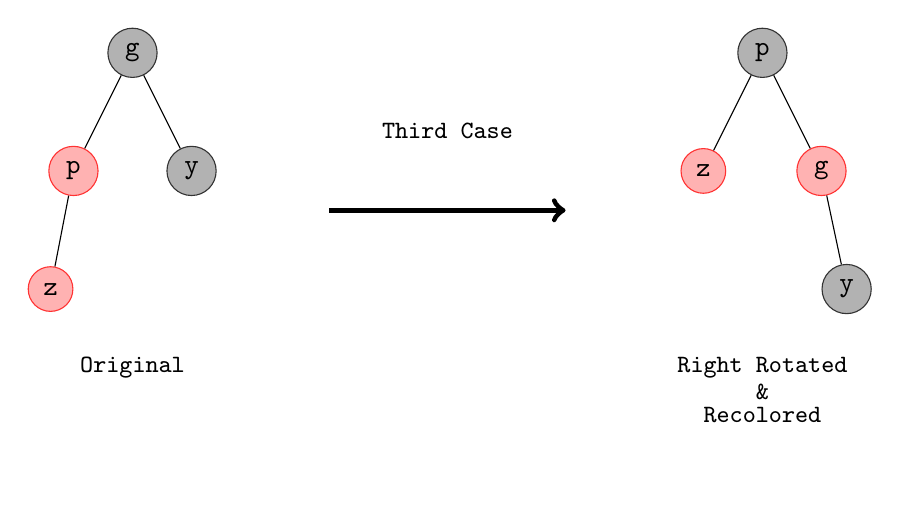
\begin{tikzpicture}[
          level distance=15mm, sibling distance=15mm,
          every node/.style={circle, draw, minimum size=8mm, font=\ttfamily\small}
        ]
        
        \begin{scope}[xshift=-4cm, every node/.style={circle, draw=blue!80, fill=blue!20, font =\ttfamily}]
            \node[circle, draw=black!80, fill=black!30] {g}
                child {node [circle, draw=red!80, fill=red!30]{p}
                    child[left] {
                        node [circle, draw=red!80, fill=red!30]{z}
                    } 
                }
                child{node[circle, draw=black!80, fill=black!30]{y}}
            ;
        \end{scope}
        
        \begin{scope}[xshift=+4cm, every node/.style={circle, draw=blue!80, fill=blue!20, font=\ttfamily}]
            \node[circle, draw=black!80, fill=black!30] {p}
                child {node [circle, draw=red!80, fill=red!30] {z}}
                child {node [circle, draw=red!80, fill=red!30] {g}
                    child[right] {
                        node [circle, draw=black!80, fill=black!30]{y}
                    } 
                };
        \end{scope}
        
        \draw[->, very thick, line width=2pt] (-1.5,-2.0) -- (1.5,-2.0) 
            node[midway, above, yshift=0.2pt, draw=none, fill=none] {Third Case};
                
        \node[draw=none, fill=none] at (-4, -4) {\textbf{Original} };
        \node[draw=none, fill=none] at (4, -4) {\textbf{Right Rotated}};
        \node[draw=none, fill=none] at (4, -4.3) {\textbf{\&}};
        \node[draw=none, fill=none] at (4, -4.6) {\textbf{Recolored}};
        
        \end{tikzpicture}
        \end{center}

        \end{itemize}
        \item \underline{\textbf{Function Insert:}} 
        
        Similar to the other implementations, the \texttt{Insert} function for the RBT handles two cases: if the word already exists in the tree, it simply adds the document ID to the list. Otherwise, it adds a new node as a leaf. For the RBT, at the end of this process, the tree is rebalanced using the \texttt{FixInsert} function.
    \end{itemize}        






    
